\chapter{Introduction}
The rising popularity of video games has transformed them from niche entertainment into a mainstream medium. As a result, game development has attracted a diverse audience, including enthusiasts with limited programming experience. To meet the growing demand for accessible game development tools, various frameworks and platforms have been developed. Their goal is to simplify the process, helping developers bring their visions to life without the need for advanced coding skills.

One genre that holds a special place in gaming history is point-and-click adventure, which emerged in the early 1980s and continues to influence the industry to this day. Despite its seemingly straightforward gameplay, creating a point-and-click adventure game involves implementing a variety of systems, such as a walking system, inventory mechanics, dialogue trees, and puzzle design. For inexperienced developers, designing these can be significantly difficult.

The goal of this Bachelor thesis is to design and implement a framework tailored to the development of 2D point-and-click adventure games. This framework, called \textit{TaleCraft}, will prioritize functionality, user-friendliness, and accessibility, encouraging beginner to intermediate game developers to create engaging games without requiring advanced programming knowledge. Since the goal is to streamline the development of 2D point-and-click adventure games, \textit{TaleCraft} will include all the essential mechanics of the genre, providing core systems such as movement, dialogue, and inventory management. Additionally, it will allow developers to customize these elements to fit their artistic and narrative vision. By addressing the unique challenges associated with point-and-click adventure game development, this thesis aims to provide a valuable tool for aspiring developers. To demonstrate its functionality and ease of use, a prototype game will be developed using the framework. 

To develop our framework, we will use the Unity game engine. Microsoft Visual Studio will be used to write scripts in the C\# programming language. 

We would also like to emphasize that some features will not be implemented
in the showcase of our framework. These features will be marked by the following box:
\todo{not demo game}

\newtcolorbox{notImplemented}{
center,
width=1.0\linewidth,
colframe=black!18!white,
colback=black!2!white, 
boxrule=1pt
}

\begin{notImplemented}
\quad {\footnotesize \textit{(not implemented)}} \par
\vspace{3mm}
A feature that will not be seen in the show case.
\end{notImplemented}

\section{Point-and-click adventure games}
A typical point-and-click adventure game emphasizes exploration, puzzle solving, and narrative engagement often involving mystery and exploration. Players interact with in-game environments through mouse-based controls and a cursor is used to click on objects, locations, or characters within a visual scene to trigger actions or dialogues. 

A very important aspect of this genre is the inventory system, which allows players to collect, examine, and use items to advance the story. Similarly, a dialogue system plays a major role, as conversations with non-player characters (NPCs) often provide essential information, influence story progression, or present choices that shape the outcome of the game. Additionally, character movement is typically controlled by clicking on a location, guiding the protagonist to navigate the world and interact with objects. Another defining feature is the command system, which determines how players interact with the world. Some games use a command panel with verbs such as “\texttt{Look at}”, “\texttt{Pick up}”, or “\texttt{Talk to}”, allowing players to take specific actions, while others rely solely on mouse-based interactions, where clicking on an object automatically triggers the most appropriate action. 

\subsection{History}
Early text-based video games like \textit{The Sumerian Game} (1964) introduced simple verb-noun parsers that allowed players to interact with the game world by typing commands \cite{Salter2014}[p. 29]. Building on this foundation, a notable predecessor to the point-and-click genre \textit{Colossal Cave Adventure} (1976) and games directly inspired by its legacy took the first steps toward integrating graphics into adventure gameplay. These games, while still reliant on text-based commands, used static visuals to represent the game world. This marked a significant departure from the purely text-driven interfaces of earlier adventure titles. Later, games started to implement simplified interaction systems such as command buttons (e.g. “\texttt{Look at}”), which significantly improved accessibility. Some later titles took this concept even further by eliminating the need for players to choose between commands. Instead, the game selects the appropriate action based on the context and object with which the player interacts like in \textit{Beneath a Steel Sky} (1994) \cite{Carton2023history}.

Point-and-click adventure games experienced their golden age in the late 1980s and early 1990s, with iconic titles such as \textit{The Secret of Monkey Island} (1990), and \textit{Myst} (1993) captivating players with their innovative storytelling and puzzle-solving gameplay. However, as the decade progressed, the popularity of the genre slowed \cite{Qaffas202022} with fewer mainstream releases and a shift to more niche titles such as the \textit{Nancy Drew} game series.

In recent years, the point-and-click adventure genre has undergone a renaissance. Modern titles such as \textit{Thimbleweed Park} (2017) and \textit{Return to Monkey Island} (2022) have revived interest by paying homage to the retro roots of the genre while implementing modern design elements. This resurgence has also been fueled by the cinematic storytelling approach pioneered by \textit{Telltale Games}. Their narrative-driven series brought the genre back into the mainstream spotlight. The renewed interest in point-and-click adventure games highlights their timeless appeal and presents an opportunity for new developers to explore the genre. Building on its rich legacy, aspiring game creators can reimagine and modernize these games for today's audience. This cultural revival highlights the need for accessible development tools to support and sustain the creative evolution of this genre.

\section{Common features}
\label{sec:Common features}
So far in this chapter, the importance of point-and-click adventure games as a game genre has been highlighted. Now, it is necessary to take a look at concrete examples of 2D point-and-click adventure games and specifically their prominent features and characteristics. By doing this, we can find inspiration to design and create the framework. We will look closely at the following features: Commands, Inventory, Character movement, and Dialogue.

\subsection{Commands}
\label{sec:Commands}
The defining feature of every video game is the ability to interact with this medium. Historically, early adventure games used text-based verb-noun parsers, as seen in \textit{The Sumerian Game} (1964) and later in \textit{King's Quest} (1984) where players typed commands like “\texttt{Climb tree}” to interact with the game world \cite{Salter2014}[p. 38]. With the evolution of graphics, these text-based interactions were replaced by mouse-based controls. The screens
became clickable, allowing players to point to places or objects in the environment to interact with them.  Not only did it feel more intuitive, but it also eliminated the problem of trying to figure out what exact words the game wants the player to use. So, the point-and-click adventure game genre was born. From then on, a mouse (or a touchpad) was almost a requirement when playing on a PC. However, there is not only one way to interact with the environment, and many modern 2D point-and-click adventure games implement different methods, sometimes even combining them.

\subsubsection{Command panel}
One of the main ways players can engage with the world is a \textit{command panel} (see Figure \ref{fig:C-TSoMI}). This panel, typical of games from the golden era of 2D point-and-click adventure games, consists of a variety of verbs. Typically, if the player selects a command from the panel and hovers over an object on the screen, a short sentence will be created in the upper part of the panel (\textit{The Secret of Monkey Island}) or above the mouse cursor (\textit{Thimbleweed Park}). This provides an indication to the player of what the main character is going to do. 

For example, in Figure \ref{fig:C-TSoMI}, the command “\texttt{Look at}” is selected, and then the mouse cursor is placed over a poster. This sequence of actions creates the sentence “\texttt{Look at poster}”. By following this logic, longer sentences can be obtained if we also take items in the inventory into account. 

Upon closer inspection, one can also notice that in Figure \ref{fig:C-TSoMI} the “\texttt{Look at}” button is highlighted in a yellow color. This occurs in certain instances to indicate the most reasonable way to interact with the object, such as “\texttt{Look at poster}”, “\texttt{Talk to pirates}”, and “\texttt{Open door}”.
\begin{figure}[H]
\centering
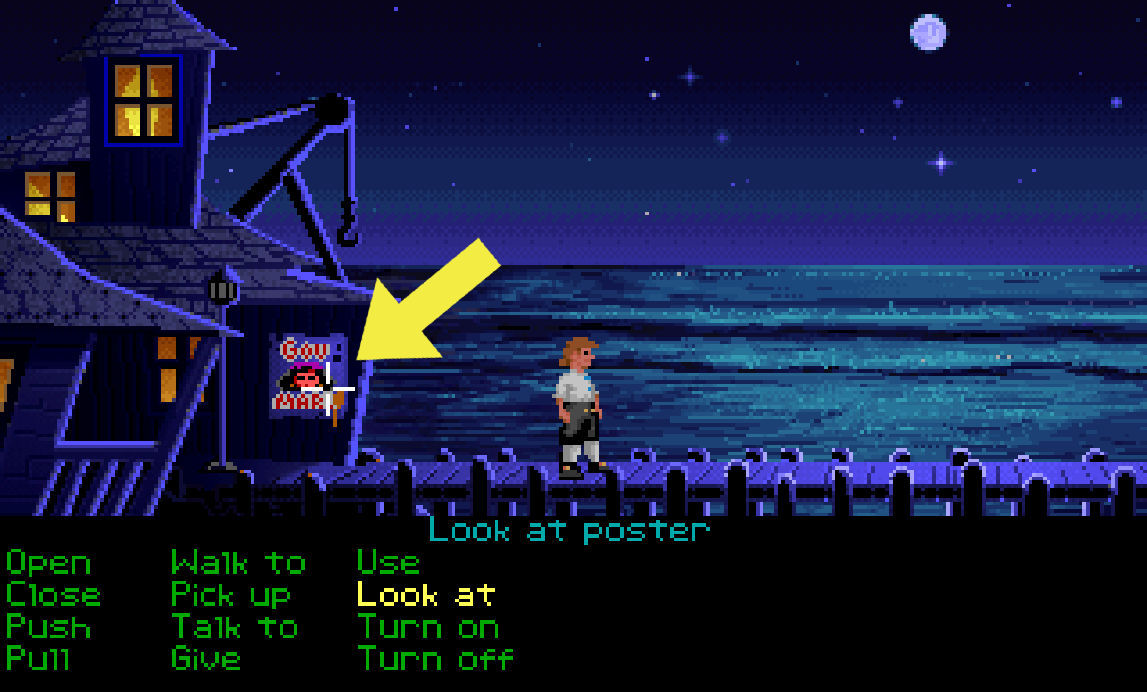
\includegraphics[width=.8\linewidth]{img/C-TSoMI.png}
\caption{The Secret of Monkey Island: Using commands and forming sentences.}
\label{fig:C-TSoMI}
\end{figure}

Most commonly, there are three forms of a sentence that can be created by combining commands and objects:
\begin{itemize}
    \item \verb|(verb)|, e.g. “\texttt{Walk to}”
    \item \verb|(verb noun)|, e.g. “\texttt{Look at poster}”
    \item \verb|(verb noun noun)|, e.g. “\texttt{Use key with lock}”
\end{itemize}
 
For each object in the game, there is a limited number of commands that have a meaningful result. Those that do not make sense for the given object result in the straightforward response something along the lines of “\texttt{That doesn't seem to work.}”  Then there are some that result in a humorous response, but do not help to progress the story either. And finally, certain panel actions help the player obtain a piece of information (“\texttt{Look at}”), change the state of an object (“\texttt{Open}”, “\texttt{Push}”, etc.), let them talk to a character (“\texttt{Talk to}”), or let them obtain or remove an item from the inventory (“\texttt{Pick up}” and “\texttt{Give}”).

\subsubsection{Mouse-based commands}
Some games are controlled by the mouse without the need for a panel of actions. Typically, the player clicks on an object with the mouse, and the game decides what to do based on the context. When hovering the mouse cursor over an object, a short text will pop up describing what that object is.

For example, in \textit{Beneath a Steel Sky} (see Figure \ref{fig:C-BaSS}), clicking with the right mouse button on an interactable object in the environment, the main character Foster will either pick it up or use it in some way (or talk to a character if that object was one). The same action with the left mouse button will result in the main character commenting about (e.g. describing) that object. If the player decides to use an item on an object, they must grab an icon using the right mouse button and then lead the item to the location of the object. Finally, if the player clicks on an empty spot that the main character can reach using either of the mouse buttons, Foster will move there. Overall, the game decides what the action will lead to.

\begin{figure}[H]
\centering
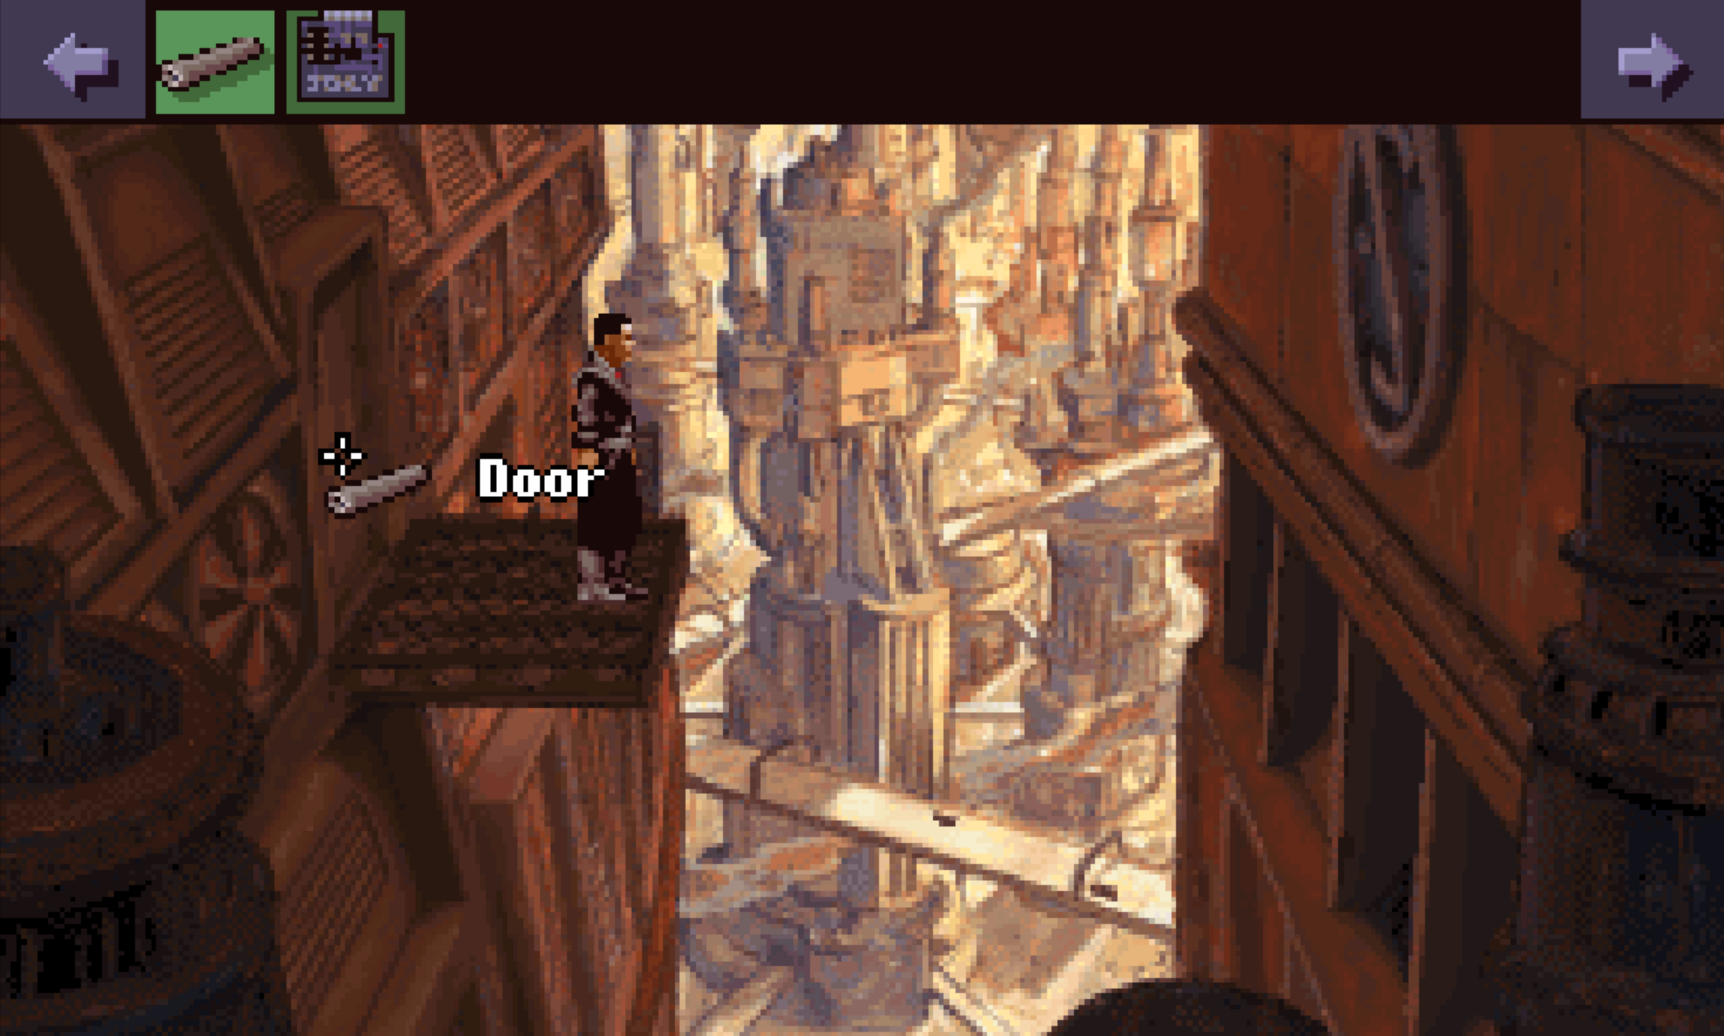
\includegraphics[width=.8\linewidth]{img/C-BaSS.png}
\caption{Beneath a Steel Sky: Using an object (a metal bar) on another object (a door).}
\label{fig:C-BaSS}
\end{figure}

As we can see, there are two different ways how a player can interact with the game's world: command panel-based interaction and direct mouse-based commands. A game designer can decide to use either (or both) of them to suit different gameplay styles, and this is what the framework should definitely support.

\subsubsection{Requirements}
To summarize, the framework should support multiple ways for players to interact with the game's world and these are the requirements:

\begin{enumerate}[label=\color{teal}\textbf{R{\arabic*}}]
  \item \label{intro:req:com_pan} The interaction can be based on a command panel, allowing structured and predefined inputs.
  \item \label{intro:req:mouse} Alternatively, players can use direct mouse-based commands for a more intuitive and hands-on approach.
  \item \label{intro:req:mix} A game designer should be able to choose either of these methods or combine them to match different styles of gameplay.
  \end{enumerate}

\subsection{Inventory}
\label{sec:Inventory}
An inventory is an integral part of most 2D point-and-click adventure games, allowing players to store, examine, and later use items to interact with the game world. The typical visual interpretation is a panel that contains a list of items that the player had collected on their journey. These can be in the form of names, which is very distinctive for games made by Lucasfilm Games in the late 1980s and early 1990s such as \textit{Zak McKracken and the Alien Mindbenders} (1988) and \textit{The Secret of Monkey Island} (1990). Another option is to have the inventory consist of icons of items. This approach has become much more popular and can be seen in most point-and-click games.

Every game handles an inventory a bit differently. In \textit{The Secret of Monkey Island}, the inventory is always visible and is located on the right side of a panel which can be found in the lower part of the screen highlighted with purple (see Figure \ref{fig:I-TSoMI}). The inventory consists of written names of the items. 

\begin{figure}[H]
\centering
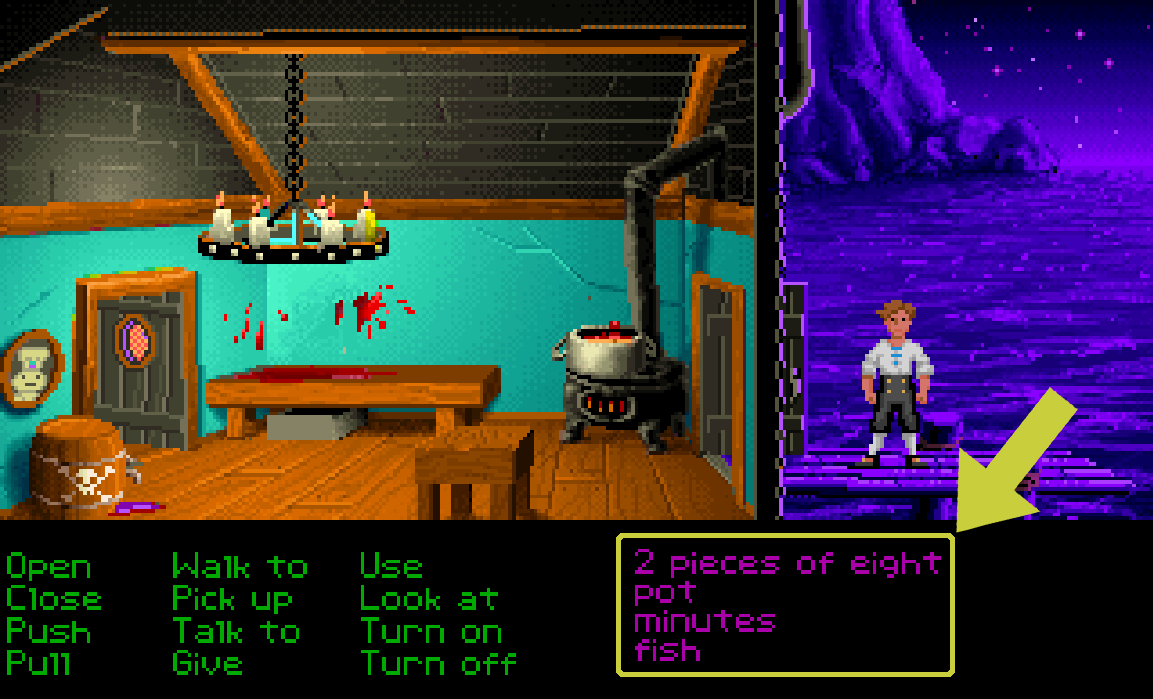
\includegraphics[width=.8\linewidth]{img/I-TSoMI.png}
\caption{The Secret of Monkey Island: Inventory}
\label{fig:I-TSoMI}
\end{figure}

To interact with items in the inventory, the game uses the \textit{command panel} just as the rest of the environment. Although this may sound obvious, this is not always true for other games. 

\textit{Fran Bow} is an example of a more modern take on the genre while still maintaining core elements from the golden era of point-and-click adventures.  A significant difference from the previous example is the fact that the inventory is completely hidden and accessible as an independent UI element in the form of a pop-up window (see Figure \ref{fig:I-FranBow}). In the game, the inventory can be opened by clicking on an icon of a purse in the lower left corner of the screen, which then displays a panel with item icons. What is also notable about \textit{Fran Bow} is the fact that its inventory uses a different command system than the rest of the game. In the game world, the player only clicks on objects, while the inventory is controlled by three buttons (see Figure \ref{fig:C-FranBow} ). 
\todo{remove one image?}

\begin{figure}[H]
\centering
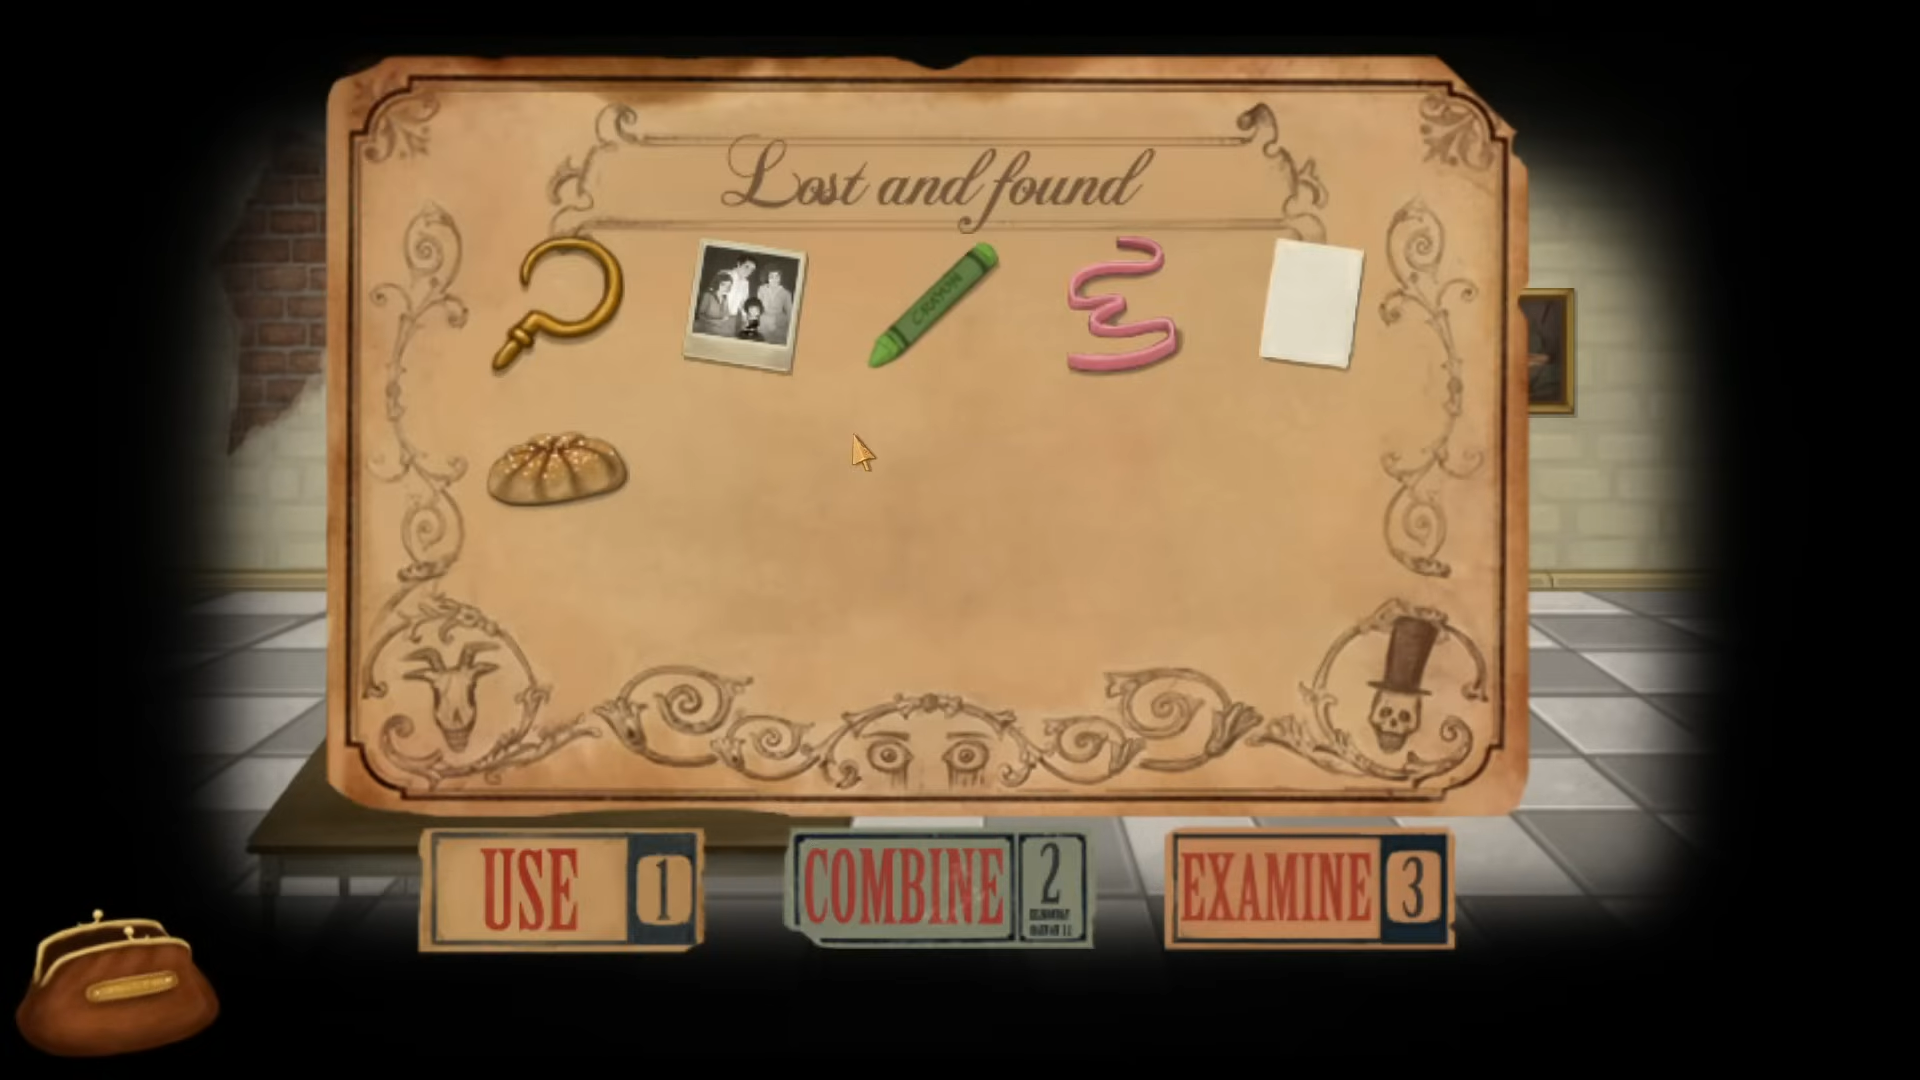
\includegraphics[width=.8\linewidth]{img/I-FB.png}
\caption{Fran Bow: Inventory}
\label{fig:I-FranBow}
\end{figure}


\begin{figure}[H]
\centering
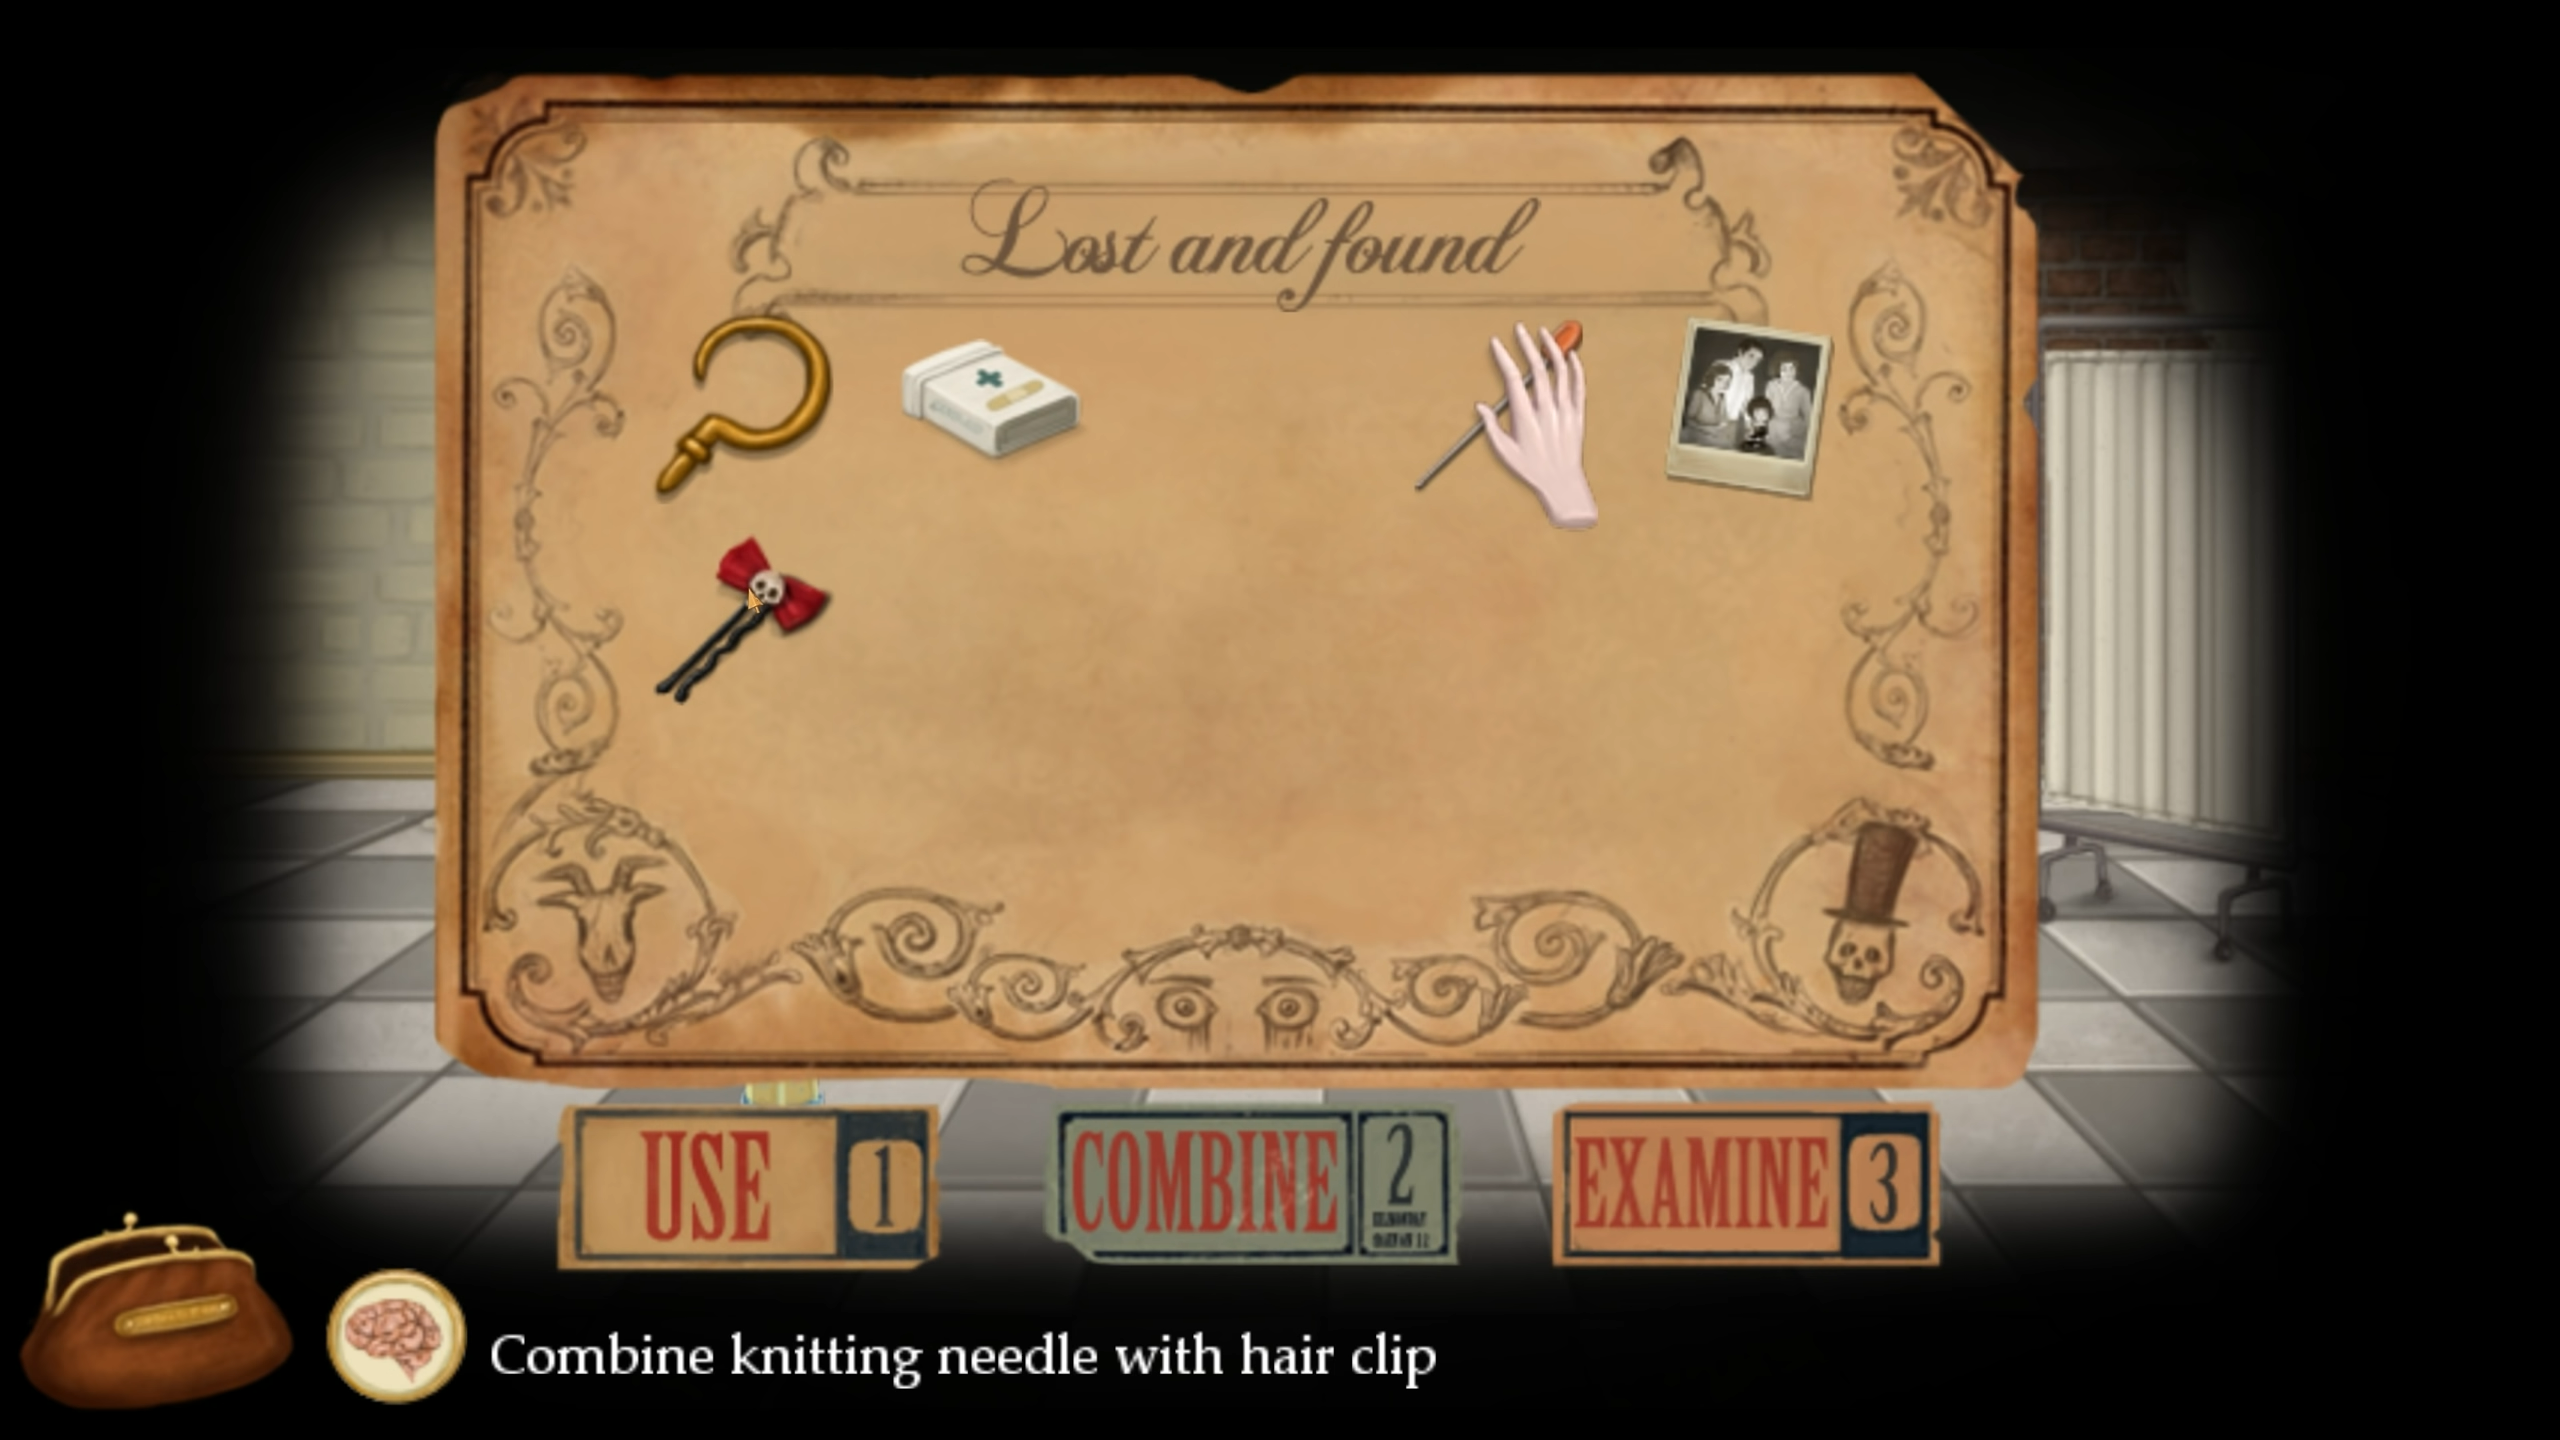
\includegraphics[width=.8\linewidth]{img/Fran_Bow.png}
\caption{Fran Bow: Combining two items in the inventory}
\label{fig:C-FranBow}
\end{figure}

Although the game uses only three commands, which is a very limited number compared to other games with similar systems, these commands are considerably more versatile. When an item in the inventory is selected and “\texttt{Examine}” is pressed, the main character Fran Bow says something about the item. In addition, there is a “\texttt{Combine}” button which allows the player to choose two items and create a new one in their place within the inventory. Finally, the third button with the “\texttt{Use}” label is a bit more versatile. Depending on the item, the player can either inspect the item closer and interact with it (e.g., unlocking a locked box and finding hidden items), or use the item outside of the inventory (e.g. giving an item to another character in the game). At the bottom of the screen, a short sentence is created according to what the player will do.

Lastly, some inventories are only partially hidden, such as the one in \textit{Beneath a Steel Sky}. The player must move the mouse cursor to the top of the screen to make the inventory panel slide down. Once visible, the player can see the icons of all items in the inventory as well as their names when the mouse hovers over an icon of a metal bar, as depicted in Figure \ref{fig:I-BaSS2}. To see a longer description, the player has to click on the item with the left mouse button. The arrows on both sides of the panel are used to navigate the inventory if it contains many items.

\begin{figure}[H]
\centering
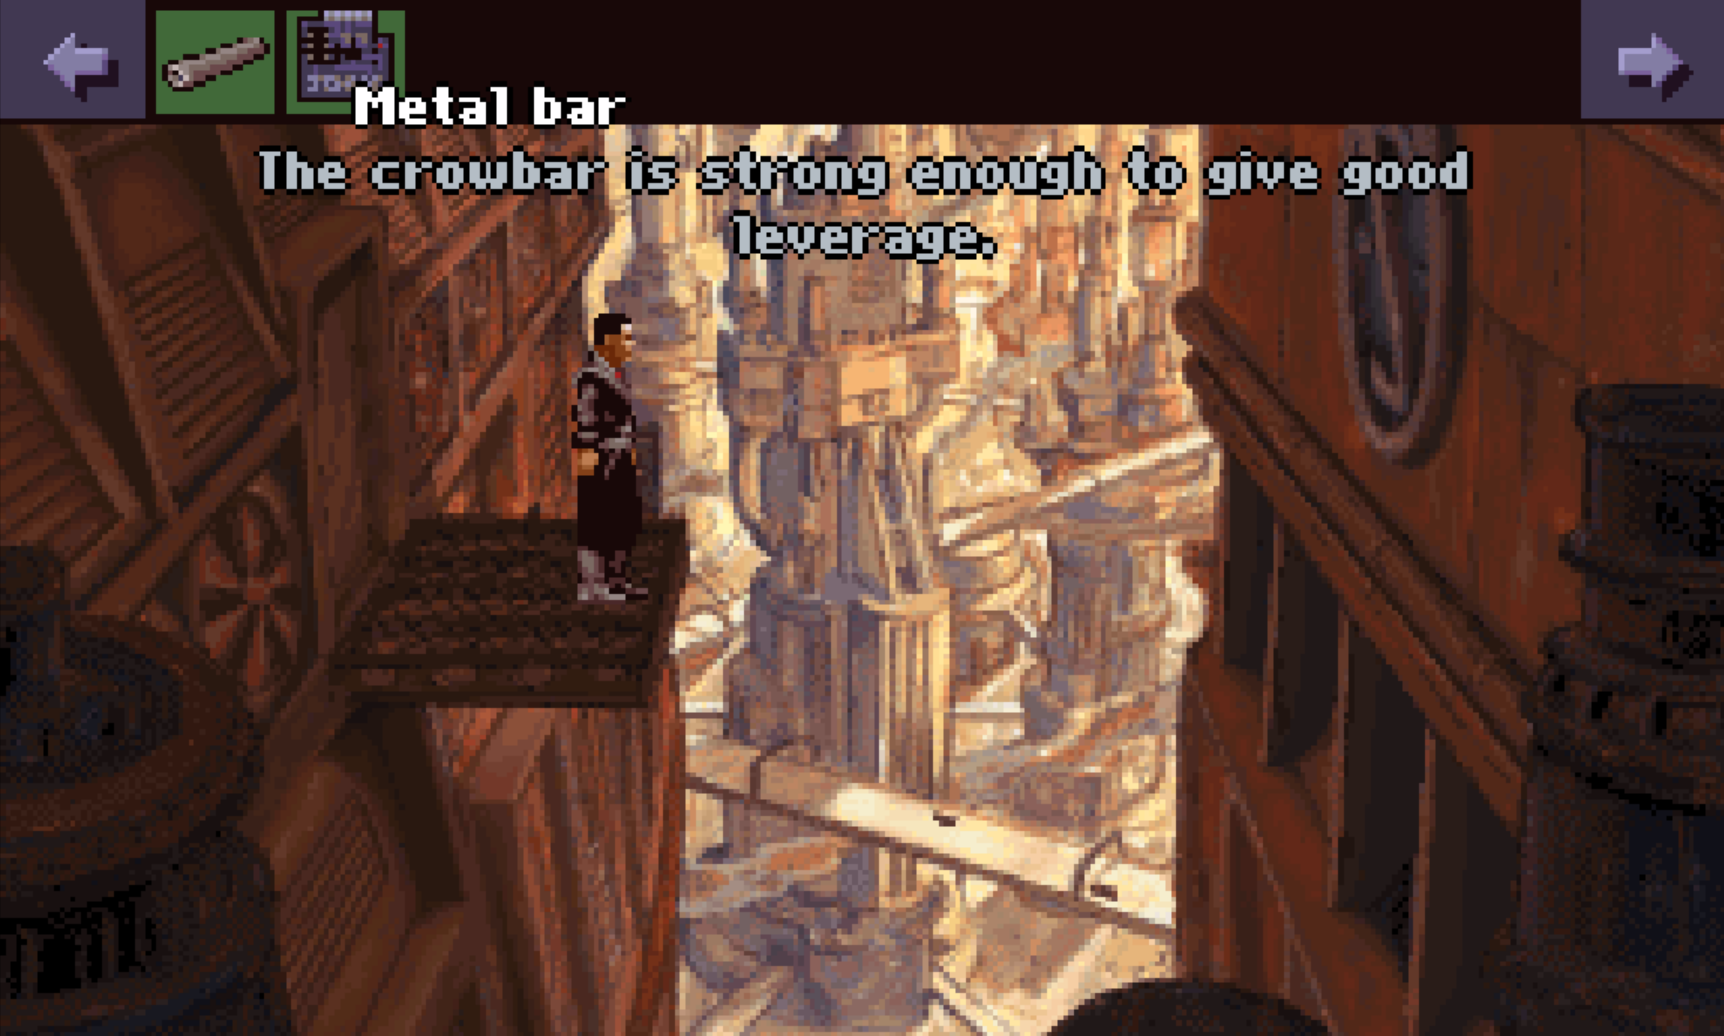
\includegraphics[width=.8\linewidth]{img/I-BaSS2.png}
\caption{Beneath a Steel Sky: Displaying a tag with the name of the item in white and a short description in grey.}
\label{fig:I-BaSS2}
\end{figure}

It is clear that the approach of games from the point-and-click genre to an inventory is very varied. That is why we want to give developers the freedom to implement it their own way by developing an inventory system that is easy to integrate and customize while supporting multiple inventory formats (static, pop-up, or sliding), including text-based lists and icon-based layouts. 

\subsubsection{Requirements}
The inventory system should be flexible and customizable. In summary, here are the requirements:

\begin{enumerate}[label=\color{teal}\textbf{R{\arabic*}},resume]
  \item \label{intro:req:inv_formats} The system should support multiple inventory formats, such as static, pop-up, or sliding inventories.
  \item \label{intro:req:text_icon} Both text-based lists and icon-based layouts should be available as inventory options.
\end{enumerate}

\subsection{Character movement}
\label{sec:Character movement}
Exploration of the in-game world is achieved through character movement. A typical way to achieve this is by clicking on a location in the environment, which prompts the character to find the shortest path and move there. The way movement is implemented can greatly impact the player's sense of control and immersion. Some games incorporate command buttons to refine the movement system. Additionally, other techniques, like character scaling, help create the illusion of depth in a 2D space to immerse the player into the game's world.

\subsubsection{Types of control}
As outlined in the previous sections, the main two ways of controlling a character either involve or do not involve the use of a command button. The one in \textit{The Secret of Monkey Island} is a prime example of the use of a command button. To move the character to another position, one must select the “\texttt{Walk to}” button and then click on a point in the environment that is not occupied by any object, as seen in Figure \ref{fig:M-TSoMI-W}. In case an object stands in that place, the character will just walk to the object without interacting with it. If there does not exist a path to the given point, the character will find the closest position to that point and walk there.

\begin{figure}[H]
\centering
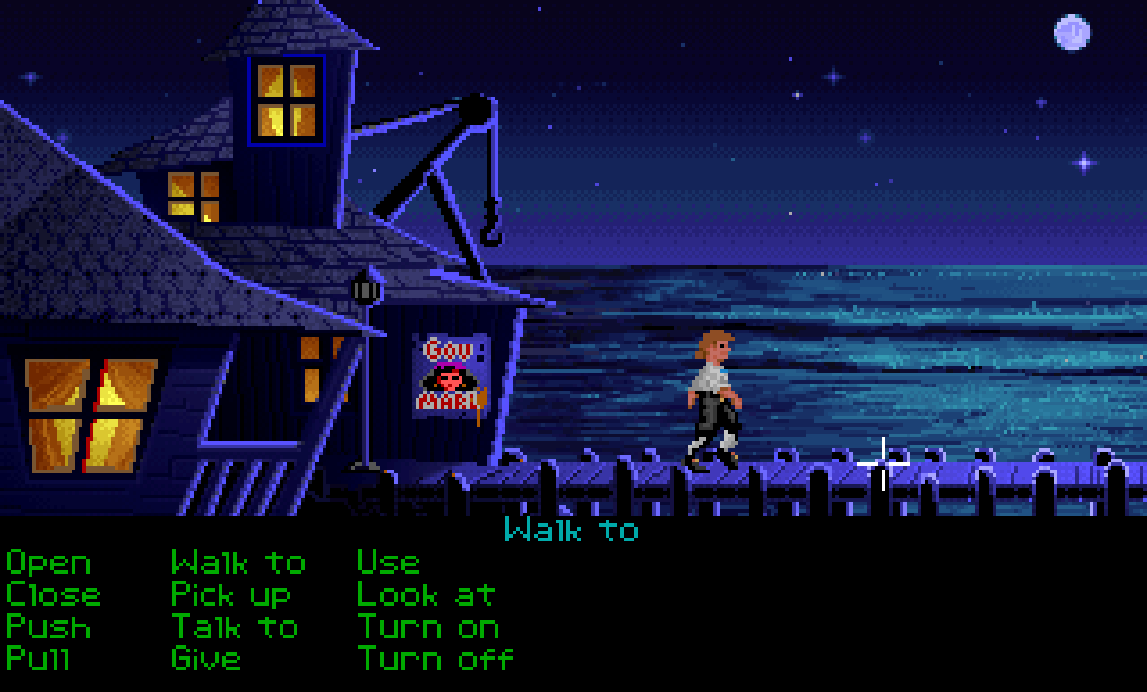
\includegraphics[width=.8\linewidth]{img/W-TSoMI.png}
\caption{The Secret of Monkey Island: Walking to a point where the mouse cursor is located}
\label{fig:M-TSoMI-W}
\end{figure}

To move the character to another position, the second option involves just clicking on a point in the environment with a mouse that is not occupied by any object. If a point occupied by an object is selected, the main character will not only walk to the point but will also interact with it as seen in Figure \ref{fig:M-BaSS}.

\begin{figure}[H]
\centering
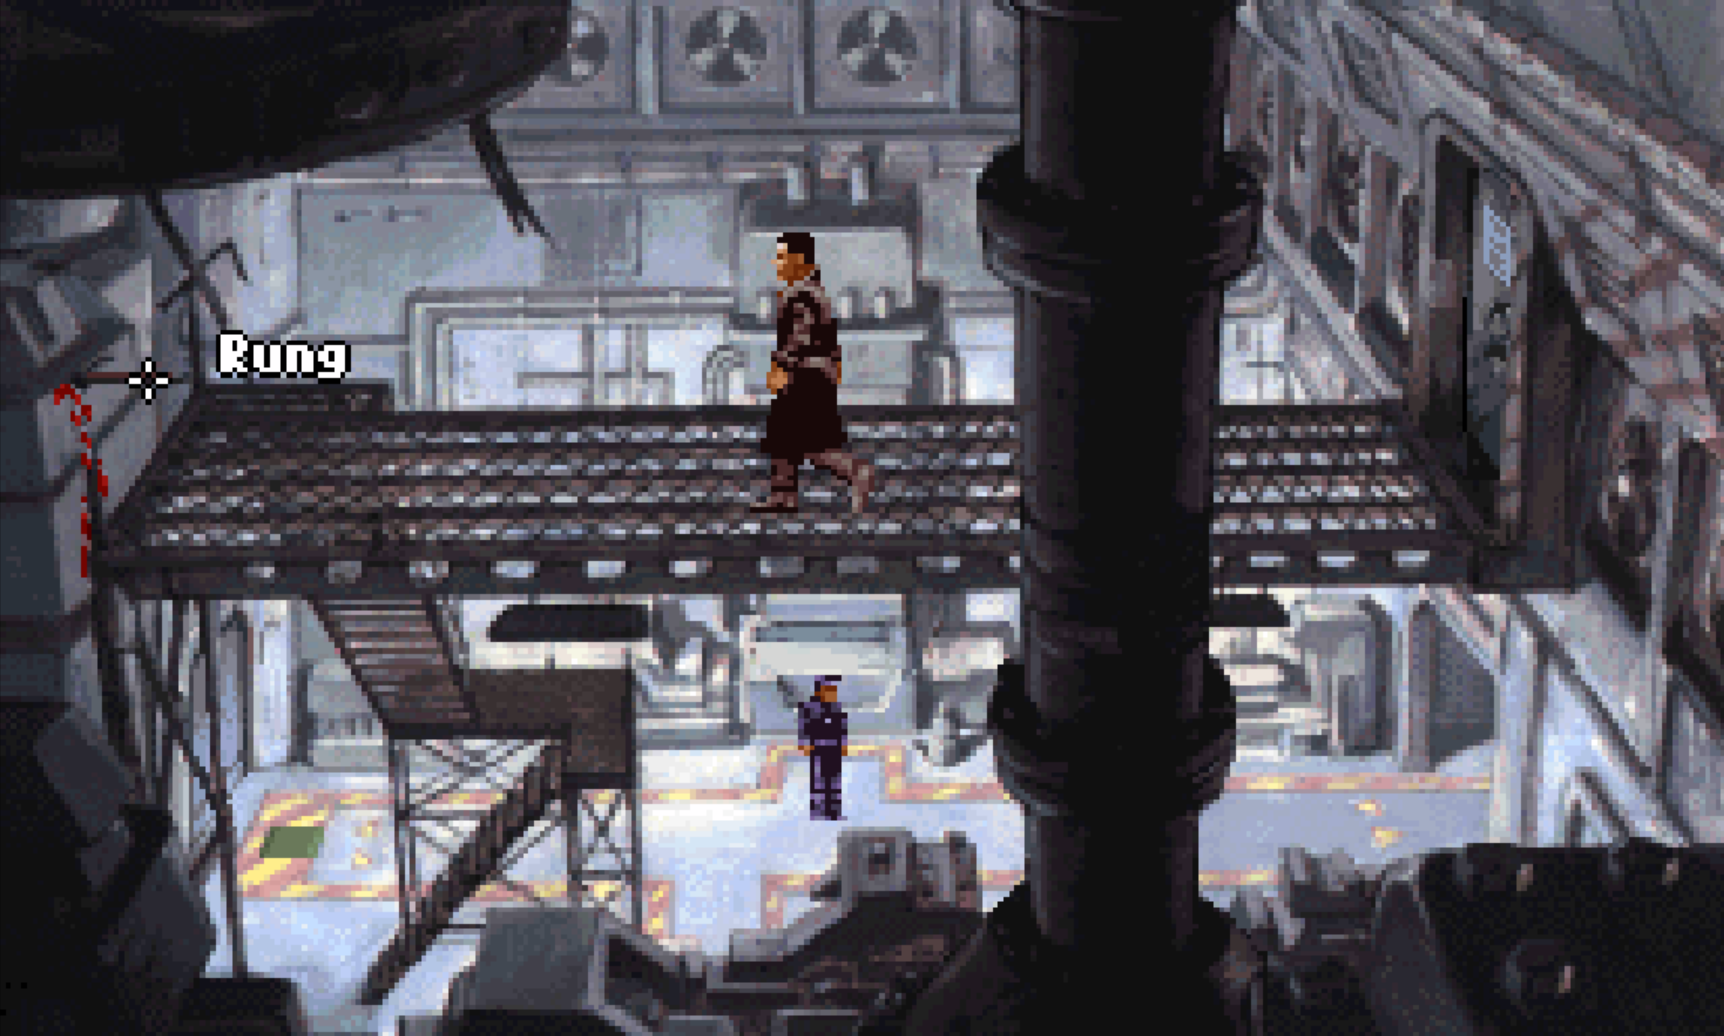
\includegraphics[width=.8\linewidth]{img/M-BaSS.png}
\caption{Beneath a Steel Sky: Walking to an object (a rung)}
\label{fig:M-BaSS}
\end{figure}

Since both types of character movement are a distinguishing feature of 2D point-and-click adventure games, we want to implement a walking system that supports both command-based movement (e.g. selecting a “\texttt{Walk to}” button) and direct mouse-based movement (clicking on a location). It is also important to have the option to specify what the end result of the movement will be, such as whether clicking on an object results in movement only or both movement and interaction. In addition to that, our aim is to incorporate pathfinding so that characters automatically navigate around obstacles to reach the desired location. 
\par
\vspace{5mm}
\textbf{Requirements} \quad In the framework, the character movement system supporting multiple interaction methods and intelligent navigation has the following requirements:

\begin{enumerate}[label=\color{teal}\textbf{R{\arabic*}},resume]
  \item \label{intro:req:com+mouse_move} Both command-based movement (e.g., selecting a “\texttt{Walk to}” button) and direct mouse-based movement (clicking on a location) should be supported.
  \item \label{intro:req:mox_move} Developers should have the option to define whether clicking on an object triggers only movement or both movement and interaction.
  \item \label{intro:req:pathfinding}Pathfinding should be incorporated so characters can automatically navigate around obstacles to reach their destination.
\end{enumerate}

\subsubsection{Depth simulation}
In some point-and-click adventure games, perspective elements are incorporated to enhance depth and spatial awareness. 
A very notable feature in some games that enhances the feeling of a 3D space is the inclusion of layers. Since the scenes in 2D point-and-click adventure games are not (usually) made using 3D spaces, the games have to simulate the appearance of objects being obscured by other objects. The difficult part comes when objects move around the scene. At one point, a character can be standing in front of an object, and then they can be standing behind the object. This means that first the character needs to be drawn above the object, and later they need to be drawn below it, just as in Figure \ref{fig:M-TSoMI0}.

\begin{figure}[H]
\centering
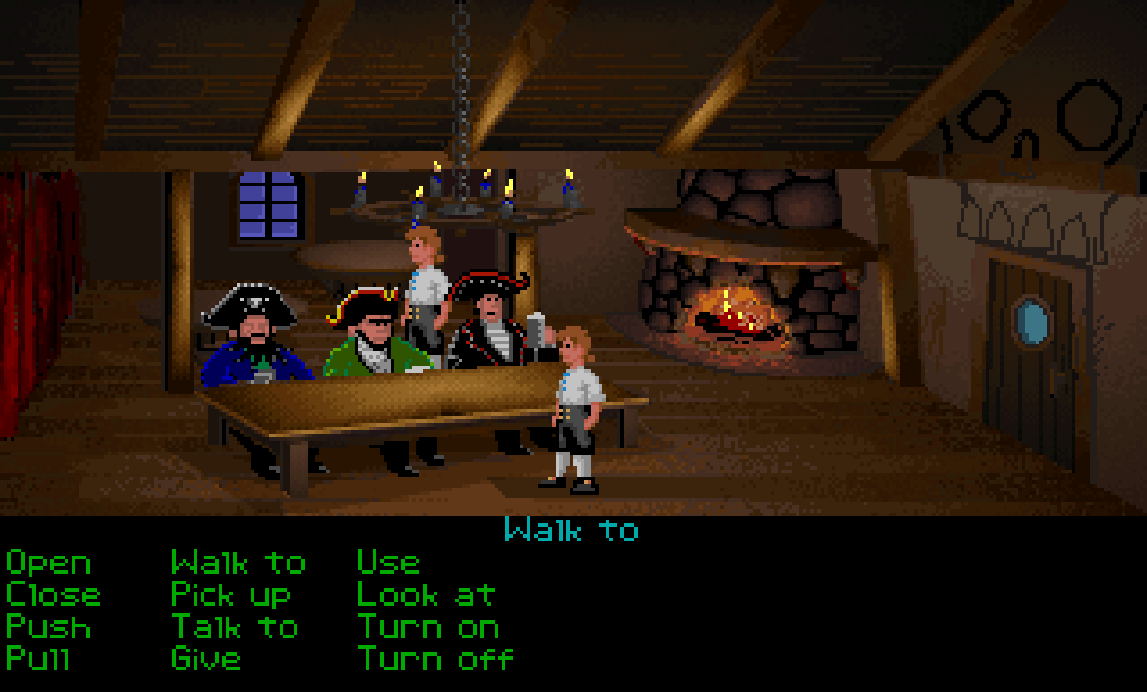
\includegraphics[width=.8\linewidth]{img/M-TSoMI0.png}
\caption{The Secret of Monkey Island: Layered composition of a 2D scene}
\label{fig:M-TSoMI0}
\end{figure}

Another way to create the illusion of a three-dimensional space within a 2D environment is making characters appear smaller as they move into the distance. One of the best examples representing this feature is in the starting area of \textit{The Secret of Monkey Island} where the main protagonist walks along the cliffside and gradually increases in size, as shown in Figure \ref{fig:M-TSoMI}. This effect can help establish a sense of scale and immersion, making the game world feel more dynamic and visually engaging. 

\begin{figure}[H]
\centering
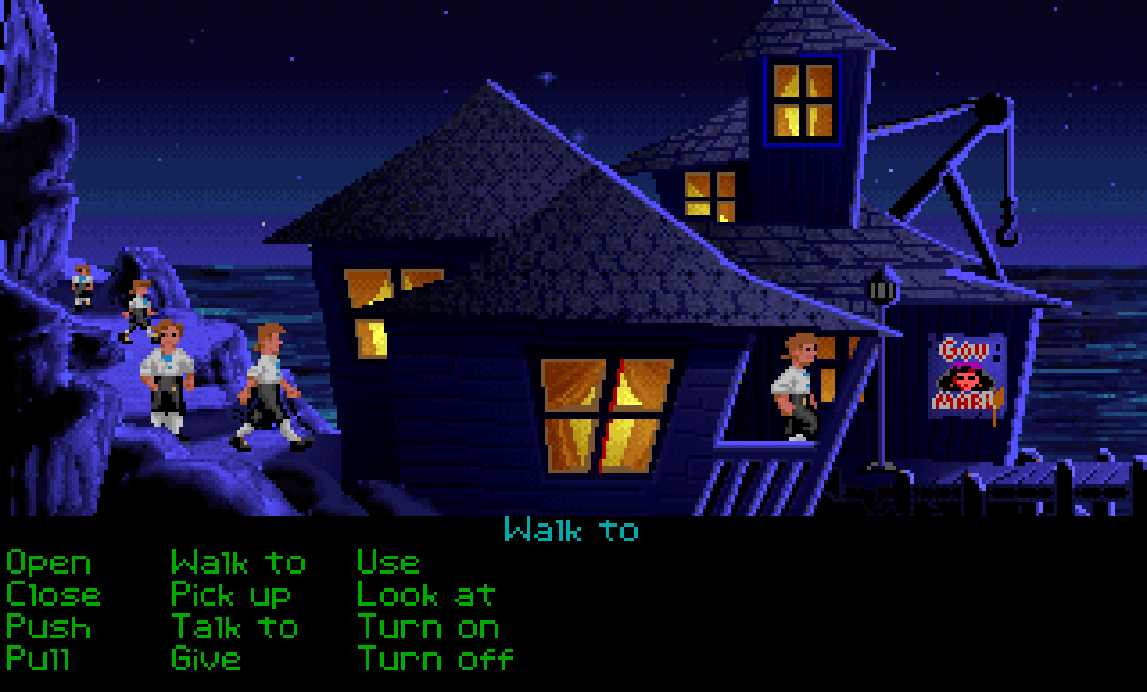
\includegraphics[width=.8\linewidth]{img/M-TSoMI.png}
\caption{The Secret of Monkey Island: Perspective simulation}
\label{fig:M-TSoMI}
\end{figure}

A similar effect was also achieved in \textit{Beneath a Steel Sky} where the main protagonist walks down a set of stairs while also being partially obscured by the platform above, which is depicted in Figure \ref{fig:M-BaSS0}.  Upon closer inspection, it appears that this process is at least partially pre-rendered in the form of a cutscene, as the player is unable to make the character move elsewhere when he reaches the staircase up until he exits it. 

\begin{figure}[H]
\centering
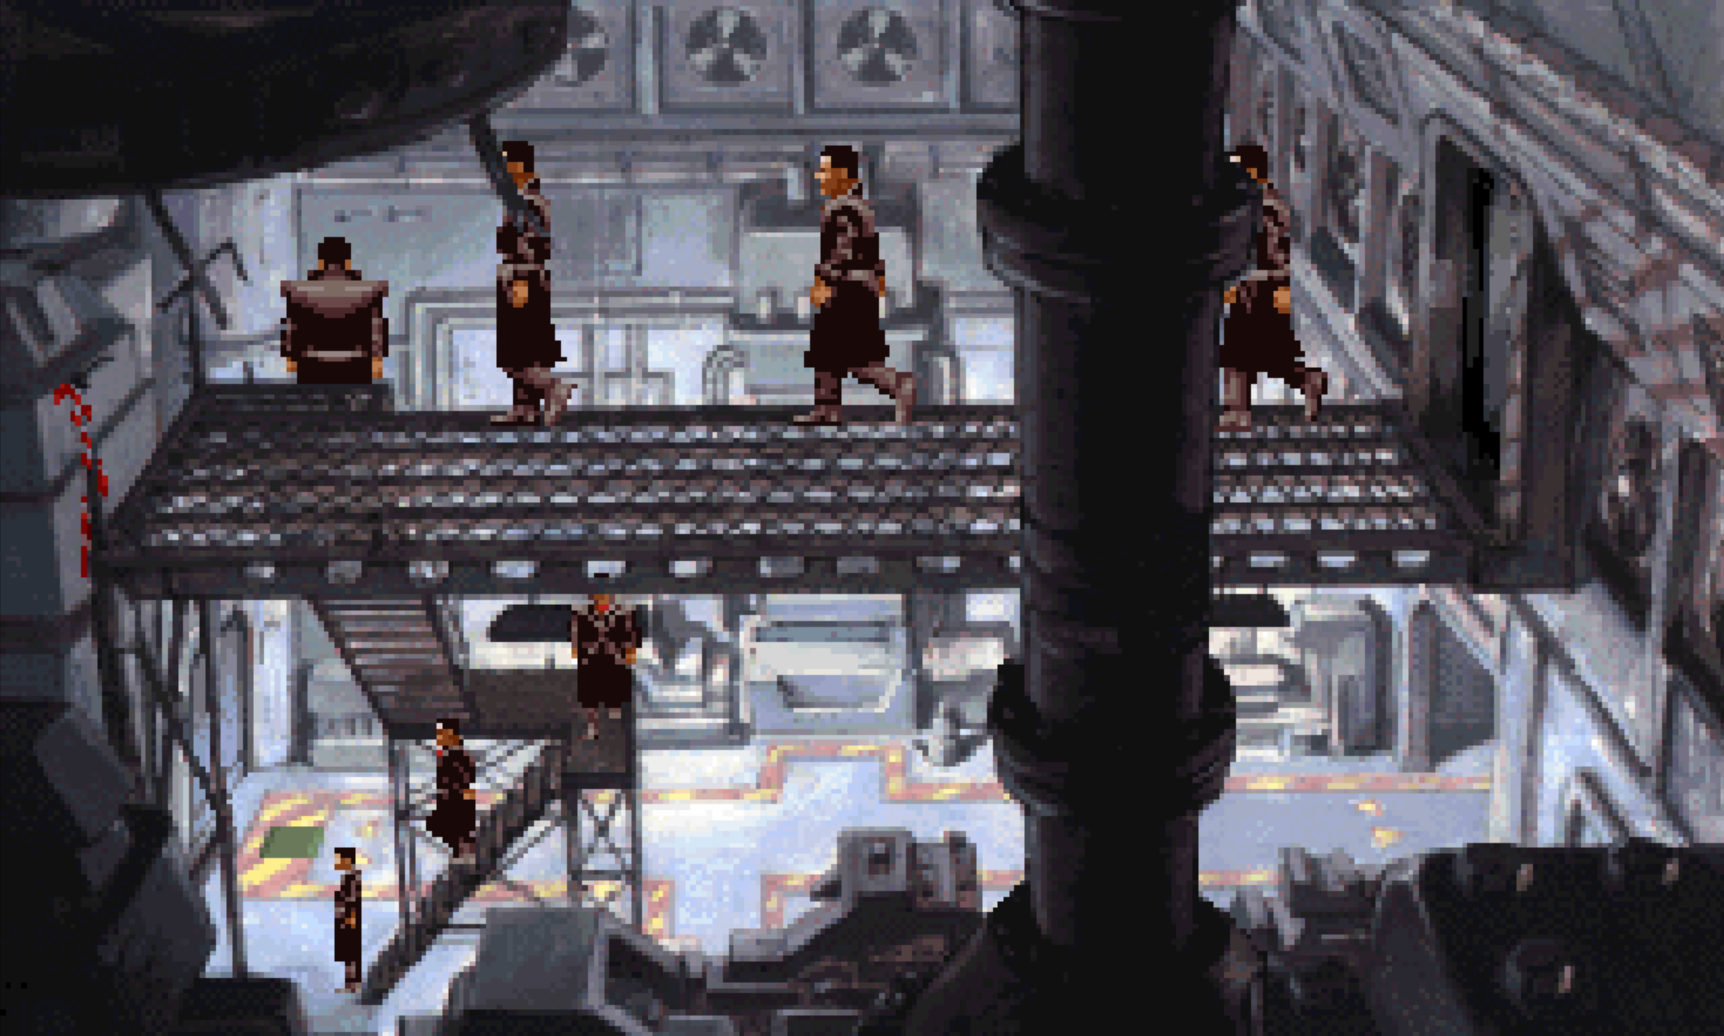
\includegraphics[width=.8\linewidth]{img/M-BaSS00.png}
\caption{Beneath a Steel Sky: Perspective simulation}
\label{fig:M-BaSS0}
\end{figure}

Dynamic and continuous character scaling, along with the ability for objects to appear in front of or behind others, plays a crucial role in maintaining the illusion of depth. To prevent the game from feeling stiff or unnatural, it is important to allow movement that preserves this 3D effect, ensuring a more immersive experience. However, some animations may be challenging to achieve just by offering the scaling and layering system. Cutscenes are often used to get around these difficult situations. However, even though cutscenes are very common in games, this thesis will not support them.
\par
\vspace{5mm}
\textbf{Requirements} \quad In summary, the illusion of depth enables the player to immerse themselves into the game's world and is achieved by the following:

\begin{enumerate}[label=\color{teal}\textbf{R{\arabic*}},resume]
  \item \label{intro:req:scale} Characters should dynamically scale to enhance depth perception.
  \item \label{intro:req:layers} Characters should adjust their position in front of or behind objects to preserve the 3D effect and to ensure a more natural and immersive experience.
\end{enumerate}
    
\subsection{Dialogue}
\label{sec:Dialogue}
Dialogues are a very important part of a 2D point-and-click game. In some examples, it is more advanced, with many options to choose from (\textit{The Secret of Monkey Island}), and in others its structure is more simple (\textit{Fran Bow}).  

In the following paragraph, we refer to terms \textit{dialogue mode} and \textit{gameplay mode} to describe how the game handles conversations. These are not standard definitions of game design. Instead, they describe the state of the games based on our observations. To initialize a dialogue with an NPC in \textit{The Secret of Monkey Island}, the player must first enter the \textit{dialogue mode} by selecting the “\texttt{Talk to}” command and then clicking on them, as shown in Figure \ref{fig:D-TSoMI0}. When done so, the dialogue starts and some features, such as the inventory, are inaccessible. Instead, the player can choose an option on how to respond to the NPC as seen in Figure \ref{fig:D-TSoMI1}. 

\begin{figure}[H]
\centering
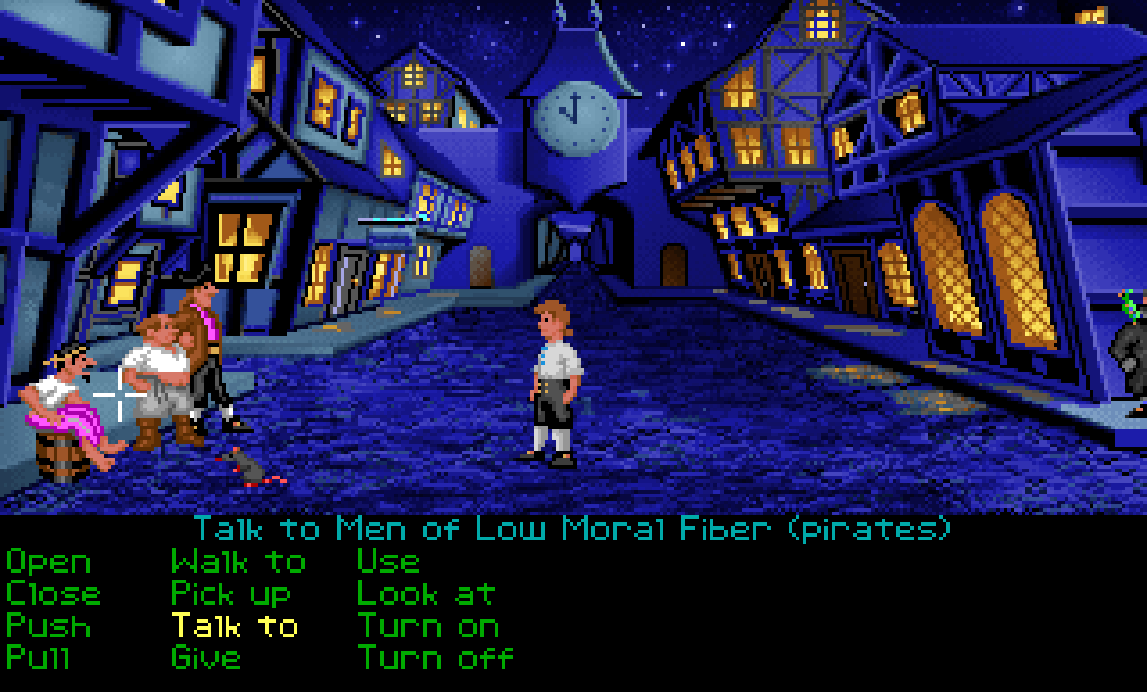
\includegraphics[width=.8\linewidth]{img/D-TSoMI0.png}
\caption{The Secret of Monkey Island: Before starting a conversation.}
\label{fig:D-TSoMI0}
\end{figure}

\begin{figure}[H]
\centering
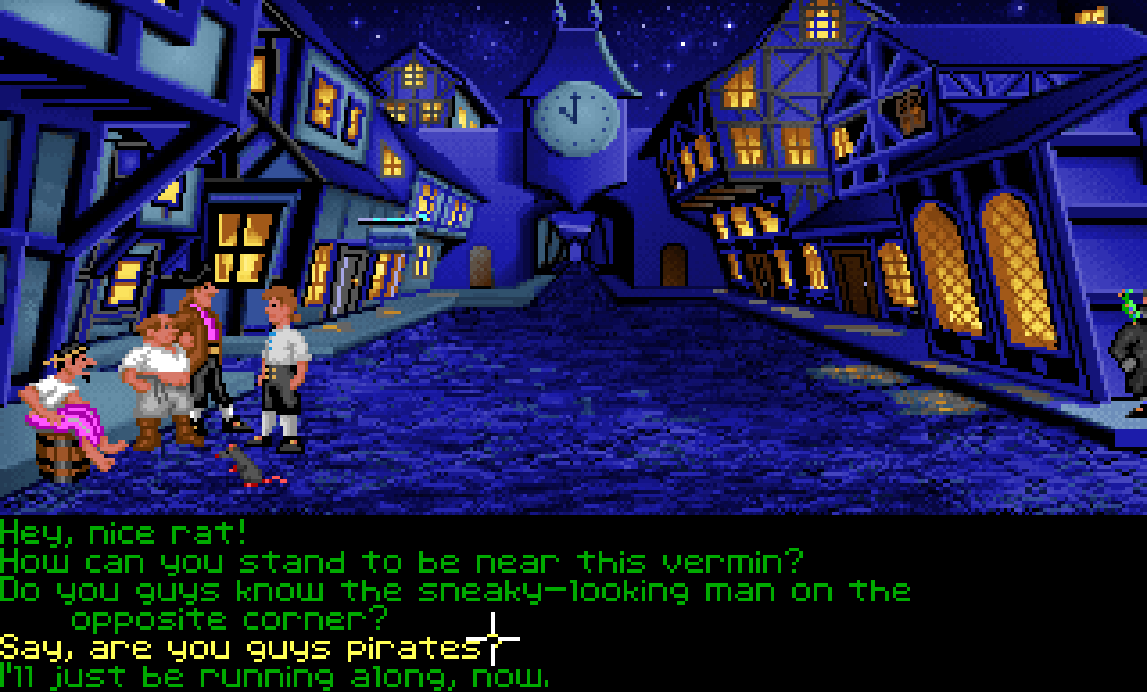
\includegraphics[width=.8\linewidth]{img/D-TSoMI1.png}
\caption{The Secret of Monkey Island: Dialogue options of the player in a conversation}
\label{fig:D-TSoMI1}
\end{figure}

By selecting the option, the player responds, and the dialogue continues until the player has the option to choose an answer again. Typically, subtitles are used to make the dialogue more accessible and understandable even with limited audio, this can be observed in Figure \ref{fig:D-TSoMI2}. To exit \textit{dialogue mode}, a specific option must be selected, and the player is back in \textit{gameplay mode}.

\begin{figure}[H]
\centering
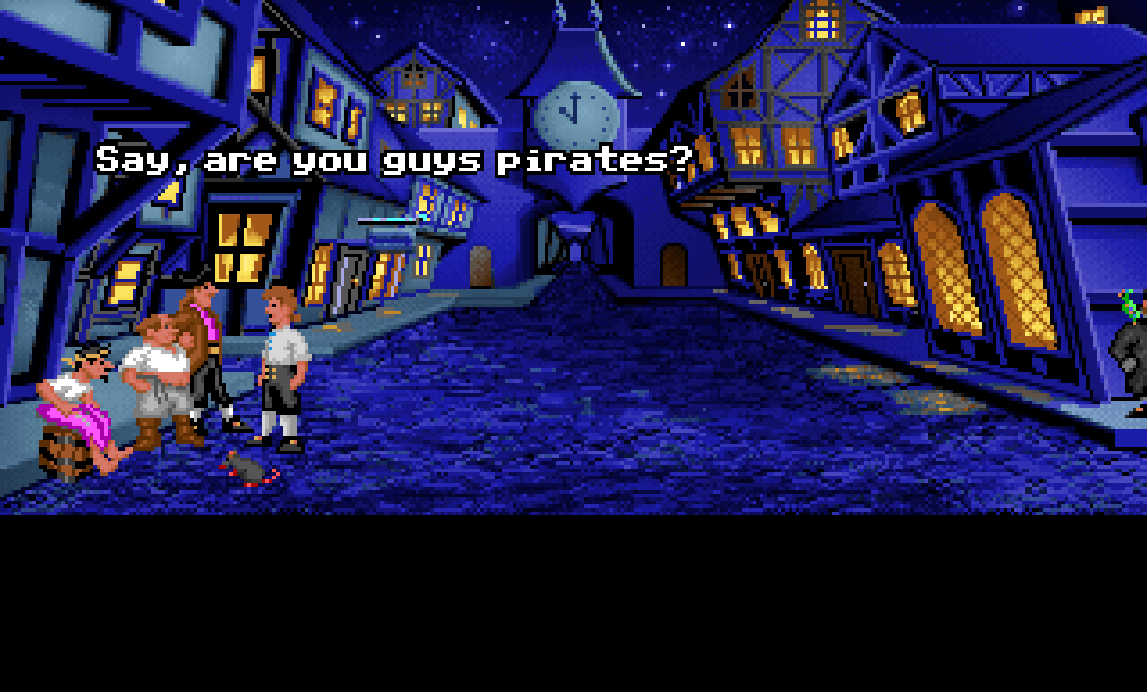
\includegraphics[width=.8\linewidth]{img/D-TSoMI2.png}
\caption{The Secret of Monkey Island: Conversation displayed through subtitles}
\label{fig:D-TSoMI2}
\end{figure}

\textit{Fran Bow} uses a similar approach. When the player clicks on an NPC, the dialogue mode is activated. As seen in Figure \ref{fig:D-FranBow}, they can interact by choosing one of two options displayed in the bottom panel. In addition, subtitles appear in bubbles above the heads of the characters. 

\begin{figure}[H]
\centering
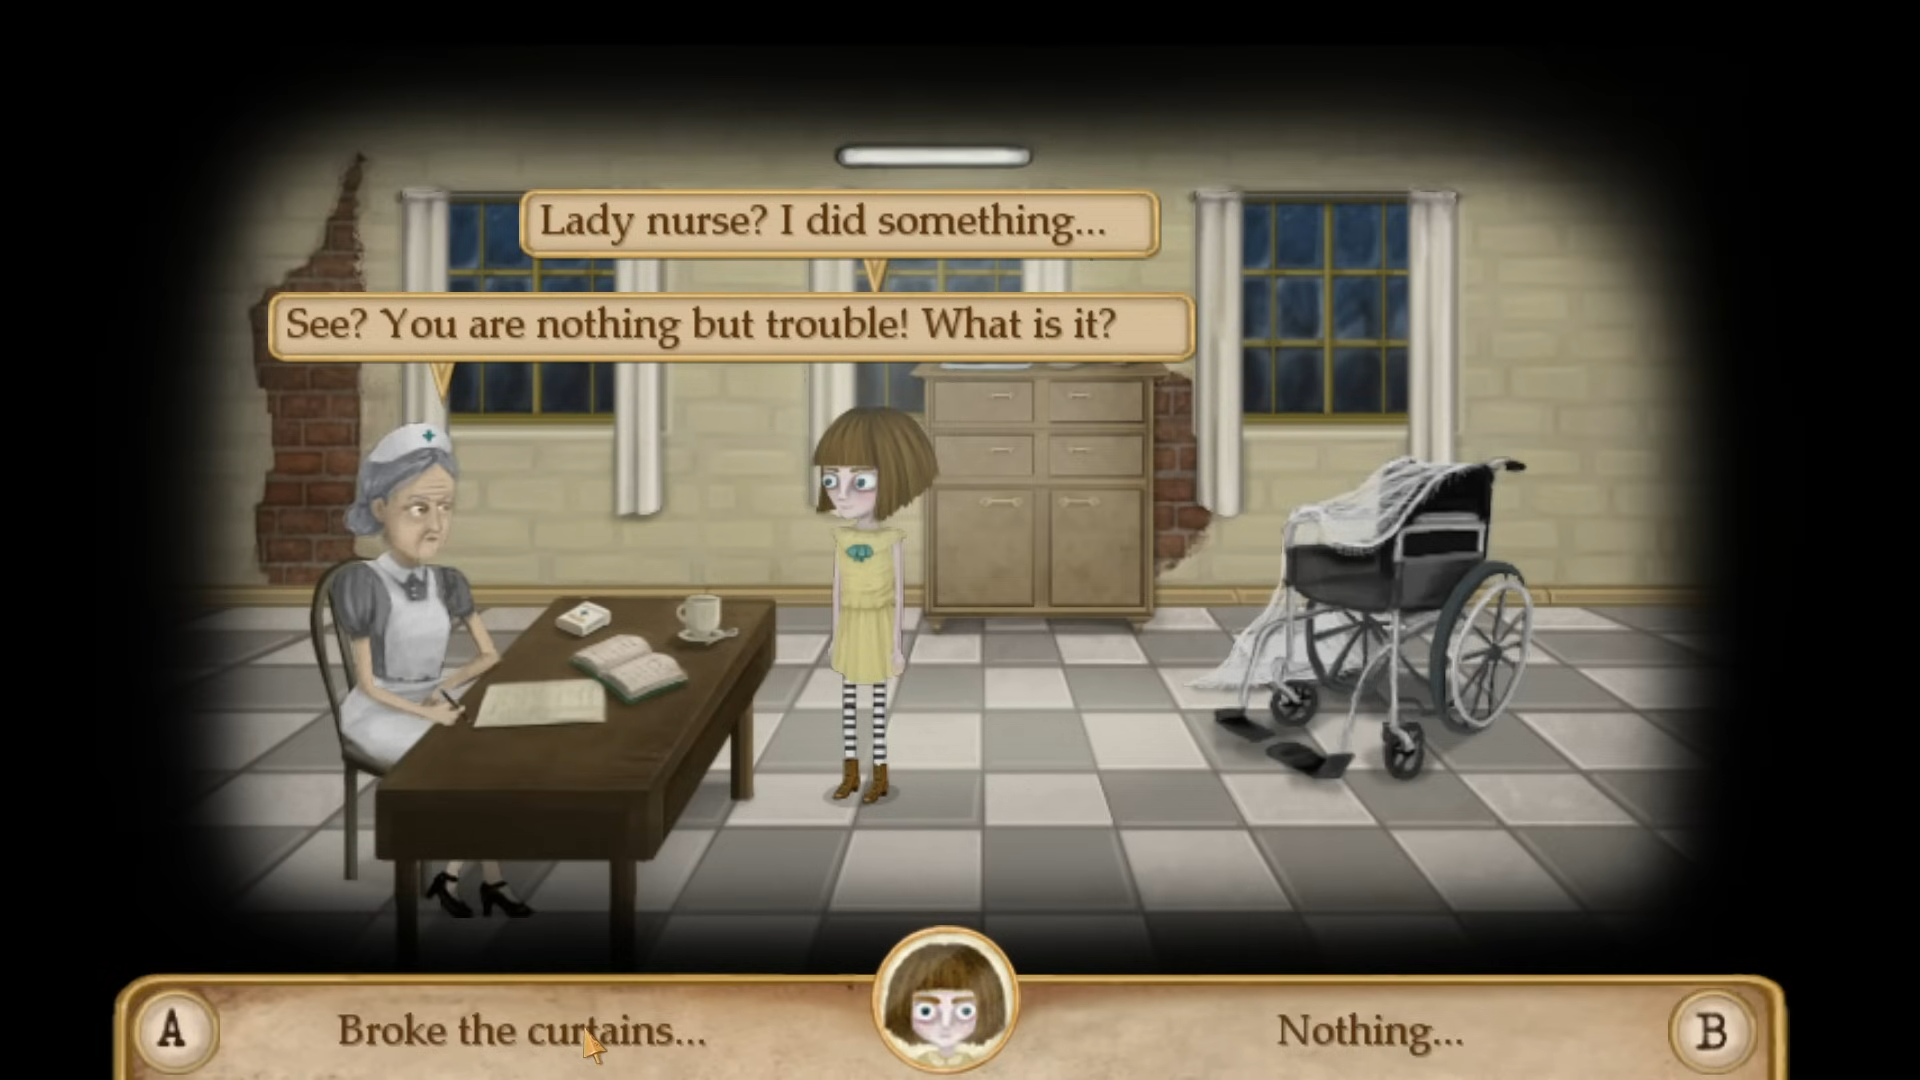
\includegraphics[width=.8\linewidth]{img/D-FB.png}
\caption{Fran Bow: Conversation with a character}
\label{fig:D-FranBow}
\end{figure}

In these two examples, the NPCs were static, so to talk to them, the character must approach them. However, this is not always the case. When examining \textit{Beneath a Steel Sky} a bit closer, one may notice that the NPCs move quite a lot around the environment and this includes also the characters player can talk to. This means that the main character must meet the character at some point on the map. \textit{Beneath a Steel Sky} solves it by determining a fixed point where the player character and the NPC must go and start the conversation depicted in Figure xxx.
\todo{include this in the project?}

Looking at these examples, the goal is clear. We want to implement a dialogue system that supports even more complex branching conversations with multiple-choice dialogue options. Next, we aim to establish a clear distinction between dialogue mode and gameplay mode, ensuring that interactions like inventory access are appropriately restricted during conversations. Finally, we want to include subtitles to enhance accessibility and improve player comprehension, regardless of audio availability, while allowing for different visual styles of dialogue presentation, such as text appearing in a dedicated panel or speech bubbles above characters. 

\subsubsection{Requirements}
To summarize, these are the rules the dialogue system should follow:

\begin{enumerate}[label=\color{teal}\textbf{R{\arabic*}},resume]
  \item \label{intro:req:multi_dialogue} It should allow for complex branching conversations with multiple-choice dialogue options.
  \item \label{intro:req:modes} There should be a clear distinction between dialogue mode and gameplay mode, restricting interactions like inventory access during conversations.
  \item \label{intro:req:subs} Subtitles should be included to improve accessibility and player comprehension, regardless of audio availability.
  \item \label{intro:req:sub_format} Different visual styles for dialogue presentation should be supported, such as text in a dedicated panel or speech bubbles above characters.
\end{enumerate}

\section{Unsupported features}
The framework could offer countless features, but the ones highlighted in the previous section represent only the core mechanics typically found in a 2D point-and-click adventure game. Many games in this genre, among others, include systems for animation, cutscenes, minigames, and sound management. However, these were not discussed as they are either not distinctive enough to be considered fundamental to the genre or fall outside the scope of this project. Naturally, the framework could be expanded in the future to incorporate these features. 
